\documentclass[14pt,a4paper]{extarticle}

\usepackage[utf8]{inputenc}
\usepackage[T1]{fontenc}
\usepackage[english]{babel}
\usepackage{fontspec}
\setmainfont{Times New Roman}

\usepackage[
    top=2cm,
    bottom=2cm,
    left=3cm,
    right=1.5cm
]{geometry}

\usepackage{setspace}
\usepackage{indentfirst}
\usepackage{enumitem}
\usepackage{booktabs}
\usepackage{longtable}
\usepackage{array}
\usepackage{hyperref}
\usepackage{xcolor}
\usepackage{titlesec}
\usepackage{caption}
\usepackage{tabularx}
\usepackage{amsmath}
\usepackage{amssymb}
\usepackage{float}
\usepackage{makecell}
\usepackage{graphicx}
\graphicspath{{figures/}}

\newcolumntype{L}[1]{>{\raggedright\arraybackslash}p{#1}}

\hypersetup{
    colorlinks=true,
    linkcolor=black,
    urlcolor=blue,
    citecolor=black
}

\onehalfspacing
\setlength{\parindent}{1.25cm}
\setlength{\parskip}{0pt}

\setlist[itemize]{leftmargin=1.5em}
\setlist[enumerate]{leftmargin=1.8em}

\titleformat{\section}{\large\bfseries}{\thesection.}{0.5em}{}
\titleformat{\subsection}{\normalsize\bfseries}{\thesubsection.}{0.5em}{}
\titleformat{\subsubsection}{\normalsize\itshape}{\thesubsubsection.}{0.5em}{}

\begin{document}

\begin{titlepage}
\begin{center}

{\normalsize
Federal Autonomous Educational Institution of Higher Professional Education\\
``National Research University Higher School of Economics''
}

\vspace{1.2cm}

{\normalsize
Faculty of Social Sciences\\
Educational Programme ``Computational Social Sciences''
}

\vspace{2.4cm}

{\normalsize
Course work on the topic:
}

\vspace{0.6cm}

{\large\bfseries
``Synthetic sample generation in the context of experimental research''
}

\vspace{1cm}

\vfill

\begin{flushright}
\begin{minipage}{0.48\textwidth}
\raggedright
\textbf{Scientific advisor:}\\
Evgeny Sedashov,\\
Programme Academic Supervisor ``Computational Social Sciences'',\\
PhD, Binghamton, \\
State University of New York
\end{minipage}
\end{flushright}

\vspace{1cm}

\begin{flushright}
\begin{minipage}{0.48\textwidth}
\raggedright
\textbf{Completed by:}\\
Maria Akhryapina,\\
Elizaveta Kuznechenkova,\\
Maria Nesterskaya\\
3rd-year students of group BVSN231
\end{minipage}
\end{flushright}

\vfill

{\normalsize
Moscow, 2026
}

\end{center}
\end{titlepage}

\tableofcontents
\newpage

\section{Introduction}

Large language models (LLMs) are increasingly discussed as tools for generating synthetic respondents, stress-testing questionnaires, and piloting experimental designs before launching costly human data collection \cite{argyle2023, horton2023, dillion2023}. In this project, LLMs are treated not as replacements for survey respondents in a substantive sense, but as instruments for \emph{synthetic sample generation} in the context of early-stage experimental research. The practical motivation is straightforward: if a model can approximate how different kinds of respondents react to alternative wordings, vignettes, and contextual cues, it may be useful for piloting the structure of a survey experiment, identifying fragile manipulations, and revealing where a design is likely to be distorted by response biases.

The project is situated in the domain of \emph{social desirability bias} (SDB). This choice is theoretically and methodologically consequential. SDB-related survey items are especially demanding for LLM-based piloting because they lie at the intersection of two response-shaping forces. First, human respondents often adjust their answers toward what is socially acceptable, normatively safe, or reputationally advantageous \cite{tourangeau2007, krumpal2013}. Second, contemporary LLMs are themselves tuned, through human-preference alignment, to avoid harmful, offensive, or normatively problematic outputs --- and there is direct evidence that this tuning produces human-like social desirability skews in survey settings \cite{salecha2024, sharma2023}. As a result, SDB is not merely one topic among many: it is a difficult test case in which the model's safety alignment may interact with the substantive logic of the survey instrument itself. If the model reproduces only sanitized, ``model citizen'' answers regardless of treatment, it is of little use as a tool for experimental pretesting in sensitive domains. If, however, it reacts systematically to experimental manipulations and carefully designed prompt stimuli, then it may help researchers understand whether a survey design can elicit meaningful variation before the design is fielded on a human sample.

\textbf{Research question.} How do large language models react to stimuli in vignette-based survey experiments on socially sensitive topics? The independent variables are (i) the original experimental treatments embedded in the vignettes and (ii) additional realism-oriented system-prompt stimuli introduced by the project; the dependent variables are the model's final survey answer, the structure of its verbalized reasoning, and its internal hidden-state representations.

\textbf{Goal.} To establish whether, and under what prompt conditions, reasoning-capable LLMs can serve as informative pilot environments for vignette experiments in SDB-sensitive domains, by tracing the effect of prompt-level interventions across three levels of observation: final answers, reasoning traces, and hidden states.

\textbf{Tasks.}
\begin{enumerate}
    \item Determine whether LLMs reproduce the direction of the original human treatment effects in two published vignette experiments (a negative-valence and a positive-valence SDB case).
    \item Estimate the effect of realism-oriented system-prompt stimuli on final answers and on the stability of those answers, and test whether the stimuli moderate the original treatment effects.
    \item Identify which design properties of the stimuli (framing valence, recipient of consequences, beneficiary, instruction force) are responsible for behavioral change.
    \item Convert reasoning traces into structured variables via LLM annotation, validate the annotation, and test how stimuli reorganize the argumentative structure of reasoning and how reasoning features relate to final answers.
    \item Test whether the stimuli are visible in the model's hidden states: at which layers stimulus information is encoded, whether treatment is encoded abstractly, and where the eventual answer becomes linearly decodable.
\end{enumerate}

\textbf{Hypotheses.}
\begin{itemize}
    \item[H1.] In the no-stimulus baseline, LLMs reproduce the qualitative direction of the original treatment effects in both experiments.
    \item[H2.] Realism-oriented stimuli shift final answers away from the socially desirable pole, with the direction of the shift depending on the normative valence of the domain.
    \item[H3.] Stimuli moderate the original treatment effects (interaction between treatment and stimulus).
    \item[H4.] Positively framed stimuli (benefit framing) produce larger departures from sanitized answering than negatively framed stimuli (penalty framing).
    \item[H5.] Stimulus effects are detectable below the surface of the final answer: in the structure of reasoning traces and in mid-layer hidden-state representations, even where the final answer does not change.
\end{itemize}

The text proceeds as follows. Section~2 reviews the literature on LLMs as synthetic respondents, on social desirability bias, and on the measurement instruments the project relies on. Sections~3--5 describe the research design: case selection, the experimental corpus, the model set, the generation protocol, and the system-prompt stimuli. Section~6 describes the reasoning-trace annotation instrument and its validation. Section~7 presents the analytical strategy, and Section~8 reports the results across the three levels of observation. Section~9 is reserved for the fine-tuned MoralLens annotation model. Sections~10--11 discuss limitations and conclude.

\section{Literature Review}

This review proceeds in four steps. First, it surveys the rapidly growing literature on LLMs as synthetic survey respondents, which defines both the promise and the known failure modes of the approach. Second, it summarizes the classical survey-methodology literature on social desirability bias, which supplies the conceptual vocabulary for the project's substantive domain. Third, it connects the two strands through recent work on social desirability and sycophancy in aligned LLMs. Fourth, it reviews the measurement instruments the project borrows from natural language processing: LLM-based text annotation and probing of hidden representations.

\subsection{LLMs as synthetic respondents}

The idea that language models can simulate survey respondents was given its canonical formulation by \cite{argyle2023}, who introduced the term ``silicon sampling'': conditioning GPT-3 on demographic backstories and showing that the resulting response distributions exhibit what the authors call \emph{algorithmic fidelity} --- fine-grained correspondence to the response patterns of the matching human subpopulations. \cite{aher2023} extended the logic from opinion distributions to experimental designs, introducing ``Turing Experiments'' that replicate classic behavioral studies (the Milgram experiment, ultimatum games, wisdom-of-crowds tasks) with simulated participants. In economics, \cite{horton2023} proposed treating the LLM as \emph{homo silicus} --- a computational implementation of an economic agent on which experimental designs can be cheaply piloted before human deployment. Perspective pieces in psychology and general science venues \cite{dillion2023, grossmann2023} frame the same opportunity more cautiously, emphasizing that LLM responses are useful precisely to the extent that their divergences from human samples are understood and measurable. At the more applied end, \cite{park2023} demonstrated that LLM-driven generative agents can sustain believable individual and social behavior over time, which broadened interest in LLM simulation beyond single-shot survey items.

A second wave of work mapped the limits of the approach. \cite{santurkar2023} showed with the OpinionQA benchmark that the opinion distributions of aligned models are skewed toward particular demographic profiles and respond only weakly to demographic steering. \cite{bisbee2024} demonstrated that synthetic survey data generated from persona prompts systematically under-disperses relative to ANES benchmarks and yields unstable regression coefficients, concluding that LLM output is not a drop-in replacement for human survey data. \cite{dominguez2024} showed that LLM answers to standard survey items are strongly driven by response-order and labeling artifacts and lack the entropy signatures of human response distributions. \cite{rottger2024} added that forced-choice formats can manufacture apparent ``opinions'' that evaporate under paraphrase. The methodological consensus emerging from this critical literature is directly relevant for the present project: LLM-based piloting is informative at the level of \emph{directional, within-design contrasts} (treatment vs.\ control under identical prompting) rather than at the level of absolute response distributions. This is exactly the standard adopted here: the project benchmarks \emph{directional replication} of treatment effects, not point estimates.

\subsection{Social desirability bias in surveys}

Social desirability bias is one of the oldest and best-documented response distortions in survey methodology. \cite{crowne1960} introduced the first widely used individual-difference measure of the tendency to present oneself in a culturally approved light; \cite{paulhus1984} decomposed the construct into two components --- self-deceptive positivity (an honest but inflated self-image) and impression management (deliberate audience-oriented adjustment) --- a distinction that remains standard. The survey-methodological literature treats SDB primarily as a property of items and contexts rather than persons: \cite{tourangeau2007} synthesize evidence that sensitive questions produce systematic misreporting whose magnitude depends on the mode of administration, the presence of an interviewer, and the respondent's perceived anonymity; \cite{krumpal2013} reviews the determinants of SDB across topic domains, showing both \emph{underreporting} of socially undesirable behaviors and \emph{overreporting} of desirable ones. Methodological work has produced both detection and mitigation tools, from the early taxonomy of coping strategies in \cite{nederhof1985} to indirect questioning designs such as list experiments, whose statistical analysis was formalized by \cite{blair2012}.

Two features of this literature shape the present design. First, SDB is bidirectional: it can push respondents toward condemnation of norm-violating behavior \emph{and} toward overstatement of virtuous behavior. The project therefore deliberately pairs a negative-valence case (support for coercive interrogation) with a positive-valence case (willingness to donate). Second, SDB operates through the response process --- through what the respondent believes the question is ``really'' asking and who will see the answer --- which motivates the project's focus on reasoning traces as a window into that process.

\subsection{Social desirability and sycophancy in aligned LLMs}

The two strands meet in recent work showing that aligned LLMs exhibit response distortions structurally analogous to human SDB. \cite{salecha2024} demonstrate that frontier models, when they can infer that they are being administered a personality questionnaire, skew their Big Five answers toward the socially desirable ends of the scales --- a direct LLM analogue of impression management. \cite{sharma2023} trace a related mechanism to the training objective itself: human-preference optimization rewards agreeable, user-pleasing outputs, producing \emph{sycophancy} --- systematic deference to the perceived expectations of the interlocutor. Together with the evidence on opinion skew under alignment \cite{santurkar2023}, this literature implies that an LLM asked a morally loaded survey question faces the same two pressures as a human respondent --- normative self-presentation and audience management --- plus a third, model-specific one: safety alignment. This is what makes the SDB domain the appropriate stress test for synthetic piloting, and what motivates the project's central intervention: system-prompt stimuli designed to reframe the model's task from self-presentation toward measurement.

\subsection{Measurement instruments: LLM annotation and probing}

The project converts reasoning traces into structured variables using an LLM annotator. The feasibility of this approach is established by \cite{gilardi2023}, who showed that ChatGPT outperforms crowd workers on standard text-annotation tasks, and by the best-practice literature \cite{tornberg2024}, which emphasizes that LLM labels must be validated against human gold-standard coding before downstream use --- a requirement the present project implements directly (Section~6.3).

For the internal-representation track, the project relies on the probing paradigm: training simple (typically linear) classifiers on intermediate representations to test what information they encode, introduced by \cite{alain2016} and critically systematized by \cite{belinkov2022}. Two methodological cautions from this literature are built into the design. First, high probe accuracy does not establish that the model \emph{uses} the encoded information; control tasks and baselines are required \cite{hewitt2019} --- the project uses permutation nulls and group-held-out cross-validation for this purpose. Second, representation-level findings gain interest when connected to behavior, as in representation-engineering work that reads and steers high-level concepts in activation space \cite{zou2023} and unsupervised latent-knowledge discovery \cite{burns2022}. For the interpretable-ML layer linking annotation features to answers, the project uses the SHAP framework of \cite{lundberg2017}, applied in a discovery-then-confirmation design (Section~8.3).

\subsection{Summary}

The literature establishes (i) that LLM simulation of survey respondents is informative for directional, within-design contrasts but unreliable for absolute distributions; (ii) that SDB is a bidirectional, process-level distortion requiring both negative- and positive-valence test cases; (iii) that aligned LLMs plausibly exhibit an SDB analogue with an additional alignment-induced component; and (iv) that both LLM annotation and probing are usable measurement instruments provided they are validated against gold labels and guarded with control baselines. The present project occupies the intersection of these four results: it uses directional replication as the benchmark, pairs opposite-valence SDB experiments, intervenes on the model's self-presentation incentives through system prompts, and measures the consequences on three validated levels --- answers, annotated reasoning, and hidden states.

\section{Research Design: Experiments and Corpus}

\subsection{Why attitude-expression experiments}

For the purposes of this project, survey experiments related to social desirability bias can be divided into three broad categories: \emph{methodological} SDB experiments (testing techniques for reducing or detecting socially desirable responding), \emph{self-report} SDB experiments (sensitive autobiographical questions), and \emph{attitude-expression} SDB experiments (evaluative judgments about externally described cases). The project focuses on the third category. Conceptually, attitude-expression designs make it easier to isolate how the model reacts to a vignette manipulation itself: the response is a judgment about an externally described case rather than a self-description, so the prompt does not need to induce a plausible autobiography. Practically, published attitude experiments have compact designs, clearly differentiated treatment conditions, and outcome measures that map onto a stable prompt template. At the same time, they remain genuinely difficult for LLMs: when the vignette concerns violence or generosity, an aligned model may drift toward a normatively polished answer regardless of treatment --- which is precisely the failure mode the project is designed to detect and counteract.

\subsection{Case selection}

The corpus consists of two published experiments selected by the following criteria: the article contains, or allows a defensible reconstruction of, the experimental conditions; the design includes multiple conditions so that treatment contrasts can be reproduced; the dependent variable is an evaluative judgment rather than self-report; the wording can be implemented in a stable prompt format across models; and the pair spans both a socially \emph{negative} and a socially \emph{positive} direction of desirability pressure. The last criterion is central: it makes it possible to study whether prompt stimuli operate symmetrically across normative valences.

\textbf{Study 1 (negative pole): coercive interrogation.} The first study reproduces the vignette experiment of \cite{hassner2022} on persuasive and unpersuasive critiques of torture. The respondent evaluates whether a terror suspect should be subjected to sleep deprivation during interrogation. Four conditions are implemented: a control base case and three treatments varying the expected informational value of the coercive act (\emph{modest intelligence}), its severity and duration (\emph{protracted duration}), and their combination. The dependent variable is binary: support for the interrogation (Yes/No, presented as numbered options 1/2). Supporting coercive interrogation is normatively problematic, so the socially desirable default is categorical rejection.

\textbf{Study 2 (positive pole): charitable donation.} The second study reproduces the donation experiment of \cite{savary2020} on unobserved altruism. The respondent evaluates willingness to donate \$5 under three conditions: a private-donation control, a public-recognition treatment, and public recognition with an added social benefit. The dependent variable is a five-point willingness scale (1 = ``Not at all willing'' \dots\ 5). Donating is socially approved, so desirability pressure here pushes toward \emph{overstatement} of willingness --- the opposite direction from Study 1.

\subsection{Prompt template and observation unit}

All runs use a fixed single-pass template. The system prompt instructs the model: \emph{``You are answering as a plausible survey respondent in a vignette-based study \dots\ Consider how a plausible respondent would evaluate this situation. Then choose exactly one response option. Output only the number of the selected option.''} The user prompt contains the vignette text, the question, and the numbered response options. Experimental treatments enter through the vignette text; the system-prompt stimuli described in Section~5 are appended to the system prompt. No demographic profile is injected into the prompt: the synthetic respondents are deliberately ``blank,'' so that all variation is attributable to the manipulated inputs. Each condition is run with 50 replicates (independent generations under distinct seeds); the replicate index plays no substantive role and serves only to quantify the stability of the response distribution.

From each single generation the project collects two outputs simultaneously: the \textbf{final answer} required by the survey instruction and the \textbf{reasoning trace} produced by the model on the way to that answer. The study does \emph{not} use a two-stage setup in which reasoning and answer are elicited separately; the final answer and the reasoning trace are two analytically distinct components of the same response event, which preserves the tightest possible link between the stated outcome and the argumentative path available for inspection.

\section{Model Set and Generation Protocol}

\subsection{Models}

The behavioral corpus is generated by four reasoning-capable models accessed through a unified API: \texttt{moonshotai/kimi-k2-thinking}, \texttt{z-ai/glm-4.6}, \texttt{qwen/qwen3.5-9b}, and \texttt{minimax/minimax-m2.5}. They were selected pragmatically rather than as an exhaustive benchmark: the project needs systems that generate not only a final answer but a sufficiently rich reasoning trace. The set nevertheless provides useful diversity in family, scale, and alignment profile, which makes cross-model comparison a substantive part of the design rather than a robustness afterthought.

A fifth model, a locally hosted \texttt{Qwen3-8B}, is used exclusively for the hidden-state track (Section~7.3): extracting layer-wise activations requires white-box access that API models do not provide. This is a deliberate design asymmetry and a known limitation --- representational findings are established on a model that is related to, but not identical with, the behavioral set.

\subsection{Generation settings}

Main generations are run at temperature $0.01$. The purpose is not to claim that near-deterministic decoding is behaviorally ``natural,'' but to maximize reproducibility at the piloting stage: since the design compares subtle differences induced by vignette treatments and system-prompt stimuli, reducing sampling noise makes the effect of the manipulated inputs easier to attribute. In addition, a dedicated baseline of no-stimulus runs was collected at temperature $1.0$ (1{,}400 rows). This high-temperature baseline serves as a methodological yardstick: it allows the project to compare the footprint of a \emph{semantic} intervention (a stimulus) against the footprint of a mere \emph{decoding-settings} change of comparable scale (Section~8.3).

\subsection{Corpus size and structure}

The assembled master table contains 15{,}680 runs: 4 models $\times$ 2 experiments $\times$ (4 or 3) treatment groups $\times$ stimulus conditions $\times$ 50 replicates, plus the temperature-1.0 baseline. After preprocessing --- removal of non-reasoning runs, deduplication via rerun patches, and exclusion of empty or unparseable answers --- the analytical dataset contains 12{,}434 rows (79.5\%). One preprocessing finding is substantive in itself: \texttt{qwen3.5-9b} refuses (returns empty responses) in 41.3\% of its runs, concentrated in the no-stimulus and balanced-stimulus conditions, whereas the other three models refuse in $\le$0.05\% of runs. Refusal is itself an alignment behavior, and its asymmetry across models is part of the heterogeneity the project documents.

One structural imbalance must be stated explicitly: the extended stimulus family H--M (Section~5) was run only on GLM-4.6 and Kimi; Minimax and Qwen3.5 cover only the no-stimulus, A, and C conditions. All analyses involving H--M are therefore estimated on the GLM+Kimi subsample and interpreted conditionally on it.

\section{System-Prompt Stimuli}

\subsection{Design logic}

The main experimental intervention introduced by the project --- beyond the vignette treatments inherited from the source studies --- is a set of \emph{system-prompt stimuli} appended to the system prompt. Their shared purpose is to reduce sanitized answering and push the model toward \emph{behavioral realism}: approximating how a plausible respondent would actually answer, rather than how an idealized moral agent ought to answer. In SDB-related settings a model may respond in a way that is safe, cautious, and normatively polished but methodologically unhelpful; the stimuli reframe the task from self-presentation toward measurement.

The stimuli form a structured design space rather than an ad hoc collection. Three dimensions are varied: (i) the \textbf{force} of the instruction --- whether it warns about consequences harshly or balances the realism request with an explicit anti-overcorrection clause; (ii) the \textbf{recipient of the consequences} of unrealistic answers --- the researcher's scientific work, science as a public enterprise, a company, or the users of its product; and (iii) the \textbf{valence of the framing} --- negative (harm if answers are unrealistic) versus positive (benefit if answers are realistic). These dimensions are miniature theories about which properties of a meta-instruction matter for an aligned model, and Section~8.1 estimates their effects directly.

\subsection{Stimulus inventory}

Table~\ref{tab:stimuli} lists the eight stimuli used in the behavioral corpus. Stimuli H--M form a (partial) factorial over the recipient/beneficiary/valence dimensions; A and C are the core-realism family in harsh and balanced variants.

\begin{longtable}{L{4.5cm} L{8.5cm}}
\caption{System-prompt stimuli in the behavioral corpus}\label{tab:stimuli}\\
\toprule
\textbf{Name} & \textbf{Core logic} \\
\midrule
\endfirsthead

\toprule
\textbf{Name} & \textbf{Core logic} \\
\midrule
\endhead

\makecell[l]{A\_original\_core\_\\realism} &
Strong realism instruction with negative consequences for the researcher if responses look sanitized rather than human. No anti-overcorrection clause. \\

\makecell[l]{C\_balanced\_\\realism} &
Same core realism instruction, with an explicit warning not to overcorrect toward provocative or implausibly extreme answers. \\

\makecell[l]{H\_science\_\\personal\_gain} &
Negative framing: the researcher's scientific work suffers if unrealistic answers reduce the informativeness of the study; anti-overcorrection clause. \\

\makecell[l]{I\_science\_\\public\_good} &
Negative framing: lower scientific value for broader public understanding; anti-overcorrection clause. \\

\makecell[l]{J\_company\_\\personal\_gain} &
Negative framing: firm-level losses if misleading data distort product design; anti-overcorrection clause. \\

\makecell[l]{K\_company\_\\public\_good} &
Negative framing: reduced usefulness of the product for real people; anti-overcorrection clause. \\

\makecell[l]{L\_science\_public\_\\good\_positive} &
Positive framing: realistic responses improve scientific value and produce a more truthful picture of human behavior. \\

\makecell[l]{M\_company\_personal\_\\gain\_positive} &
Positive framing: realistic responses improve product design and benefit the company. \\

\bottomrule
\end{longtable}

The configuration files additionally define several stimuli (softened realism, research-purpose framing, stronger stakes, scientific integrity, measurement neutrality) that were not fielded in the behavioral corpus; four of them (B, D, F, X) were used in the separate hidden-state track (Section~7.3), whose local-model runs cover the conditions $\{$none, A, B, C, D, F, X$\}$.

\section{Reasoning-Trace Annotation}

\subsection{Why reasoning traces require a dedicated instrument}

Because each run yields a reasoning trace alongside the final answer, the project needs a principled way to transform long free-form text into structured analytical variables. Raw traces are rich but unwieldy: they contain explicit moral arguments, hedging, meta-commentary on the survey format, treatment uptake, stimulus uptake, and artifacts of alignment behavior. Manual inspection during instrument development showed that the relevant features fall into two broad groups: \emph{format-related} features (reflections on the answer scale, the respondent role, what would ``look too saintly'') and \emph{substantive} features (which moral categories the model invokes, where it locates the treatment, whether it reacts to the stimulus). The coding scheme was built to preserve both layers.

\subsection{Annotation pipeline and schema}

The main annotation was produced by \texttt{gpt-5.4-mini} acting as an LLM coder. The annotator receives the experiment context (system prompt, vignette, treatment, stimulus where present) together with the full reasoning trace and returns a strictly machine-readable record conforming to a fixed schema. Two batches of 5{,}040 traces each were annotated (disjoint row sets), for a total of 10{,}080 annotated runs covering all four models, both experiments, the conditions $\{$no stimulus, A, C$\}$, and the temperature-1.0 baseline. After merging with the master table and filtering to parseable runs with valid answers, the working annotated sample is $n = 8{,}638$ (Hassner 5{,}085; Savary 3{,}475).

The schema contains 37 coded fields per trace: 19 \emph{causality} variables (does the category causally participate in the answer: 0 = absent, 1 = mentioned, 2 = decisive; binarized 0 vs.\ 1--2 for analysis), 15 \emph{direction} variables ($-1/0/+1$: does the category push the answer down or up), and 3 binary style markers (acknowledgment of the possibility of different opinions; moral-style reasoning; rational-style reasoning). The categories span treatment awareness, stimulus (incentive) awareness, overcorrection concern, self-enhancement, fear of negative evaluation, self-deception, reliance on majority or source, prioritization of common vs.\ private interests, personal cost, means--ends reasoning, emotional reasoning, public recognition, privacy, social reward, urgency, legality, and cruelty. For the 14 categories possessing a direction, analysis uses \emph{signed presence} (causality $\times$ direction); stimulus-effect direction is kept separate because of its high share of neutral codes.

\subsection{Validation against gold labels}

Following the best-practice requirement that LLM labels be validated before downstream use \cite{gilardi2023, tornberg2024}, the annotator was benchmarked against expert manual coding on a validation subset ($n=27$ traces). The result (Table~\ref{tab:kappa}) is deliberately reported as differentiated rather than averaged: agreement is excellent for \texttt{cruelty} and \texttt{personal\_cost\_burden}, substantial for \texttt{overcorrection\_concern}, but at chance level for several psychologically subtle categories. All downstream findings are therefore graded by the reliability of the categories they rest on: claims based on the validated categories are treated as measurement-grade, claims based on unvalidated categories as exploratory. The validation subset is small, and extending it is part of the planned MoralLens work (Section~9).

\begin{table}[H]
\centering
\caption{Annotator validation against expert gold labels ($n = 27$ traces, Cohen's $\kappa$)}
\label{tab:kappa}
\begin{tabular}{L{6.2cm} c L{5.2cm}}
\toprule
\textbf{Category} & $\kappa$ & \textbf{Verdict} \\
\midrule
cruelty & 1.00 & reliable \\
personal\_cost\_burden & 1.00 & reliable \\
overcorrection\_concern & 0.64 & substantial \\
treatment\_effect\_direction & 0.46 & moderate \\
emergency\_urgency & 0.42--0.44 & moderate \\
emotional\_reasoning & 0.06 & noise level \\
common\_interests\_prioritization & 0.00 & noise level \\
self\_deception & 0.00 & noise level \\
incentive\_awareness & 0.00 & noise level \\
\bottomrule
\end{tabular}
\end{table}

\section{Analytical Strategy}

The project observes LLM behavior on four connected levels --- final answers, reasoning traces, structured annotations, and hidden states --- and the analytical strategy mirrors this structure in three tracks implemented in three notebooks.

\subsection{Track 1: behavioral analysis of final answers}

The behavioral track proceeds from validation and descriptives to formal tests. Treatment effects within each stimulus condition are tested with $\chi^2$ tests (binary Hassner outcome) and Mann--Whitney/Kruskal--Wallis tests (Savary scale), with Holm correction within families; stimulus effects are tested analogously against the no-stimulus baseline; moderation (does the stimulus change the treatment effect) is assessed by difference-in-differences contrasts. Effect sizes are reported as Cram\'er's $V$ and Cohen's $d$. Regression analysis uses a logit (Hassner) and an ordinal logit with binary-threshold and OLS cross-checks (Savary), with treatment $\times$ stimulus interactions and model fixed effects.

Because 50 replicates within a design cell are not independent observations, all headline regressions are re-estimated with \emph{cluster-robust} standard errors, clustering on the design cell (model $\times$ group $\times$ stimulus; 96 clusters in Hassner, 72 in Savary). Additional robustness layers address quasi-separation (28/96 Hassner cells are perfectly separated; extreme-stimulus coefficients are reported descriptively, with ridge-penalized cross-checks), the failure of the proportional-odds assumption in Savary (binary and OLS codings are used alongside the ordinal model), Benjamini--Hochberg FDR across coefficient families, answer-stability metrics (modal agreement, Fleiss' $\kappa$), and replicate-level stability of treatment signs by model.

Finally, the stimulus inventory itself is treated as a design matrix: final answers are regressed on stimulus \emph{attributes} --- framing valence, recipient domain (science vs.\ company), beneficiary (personal vs.\ public), and instruction force (A vs.\ C) --- rather than on stimulus dummies, on the GLM+Kimi subsample where the full H--M factorial exists.

\subsection{Track 2: statistical analysis of annotated reasoning}

The annotation track has five components. (i) A baseline check that the annotated subsample reproduces the behavioral effects of Track 1. (ii) Category prevalence and its dependence on treatment and stimulus, with FDR-corrected per-category logit/OLS regressions. (iii) A \emph{separability benchmark}: classifiers (regularized logit and gradient boosting, stratified 5-fold cross-validated ROC-AUC) predicting from the annotation features whether a trace was generated under a stimulus, compared against classifiers predicting a mere temperature change ($0.01$ vs.\ $1.0$) on no-stimulus runs --- the latter providing a yardstick for how much ``footprint'' a non-semantic perturbation leaves in the markup. A leakage-controlled variant excludes the categories that detect the stimulus by construction (stimulus awareness, stimulus-effect direction). (iv) Models linking reasoning features to the final answer (logit for Hassner, OLS for Savary), with and without experimental-condition controls, including a non-tautological refit excluding the co-generated stated-position feature. (v) An interpretable-ML layer: a diagnostic comparison of linear versus gradient-boosting performance decides whether nonlinear attribution is warranted; where it is, TreeSHAP \cite{lundberg2017} is used in a \emph{discovery} role, and every discovered interaction is then re-estimated as an explicit term in a confirmatory regression with heteroskedasticity-robust inference.

\subsection{Track 3: hidden-state analysis}

The representational track runs on the local Qwen3-8B: 98 single-pass runs (56 Hassner, 42 Savary) across the conditions $\{$none, A, B, C, D, F, X$\}$, with last-token activations extracted at all 37 layers (4{,}096 dimensions each). The analyses are: layer-wise separation between stimulus and no-stimulus runs (standardized between/within distance, with bootstrap assessment of the peak's location and significance); probing \cite{alain2016, belinkov2022} of stimulus presence and of treatment status with leave-one-group-out cross-validation and permutation nulls \cite{hewitt2019}; representational geometry (PCA/UMAP); trajectory length across layers as a measure of late-layer ``work''; and the link between hidden-state shifts and behavioral shifts. Finally, layer-wise \emph{answer decodability} is probed with ridge regressions predicting the continuous answer (expected scale value from output logprobs) from each layer's activations under leave-one-out cross-validation, both pooled and on condition-residualized outcomes --- the latter isolating answer information beyond condition identity, since condition itself is trivially readable from the prompt text.

\section{Results}

\subsection{Behavioral level: replication, stimulus effects, and stimulus anatomy}

\textbf{Treatment effects replicate directionally (H1 supported).} In the no-stimulus baseline, all four checkable directional predictions from the source articles reproduce (Figure~\ref{fig:replication}). In Hassner, support for sleep deprivation falls from 44.6\% (control) to 12.2\% under the modest-intelligence treatment ($-32.3$~p.p.), 19.3\% under protracted duration ($-25.3$~p.p.), and 1.0\% under their combination ($-43.6$~p.p.) --- every critique reduces support, and the combined critique is by far the strongest, as in the original logic. In Savary, public recognition raises stated willingness from 3.39 to 3.73 (Cohen's $d = +0.72$), and public recognition with social benefit raises it most, to 4.09 ($d = +1.66$). Pairwise treatment contrasts are significant after Holm correction in 22/27 (Hassner) and 14/18 (Savary) tests.

\begin{figure}[H]
\centering
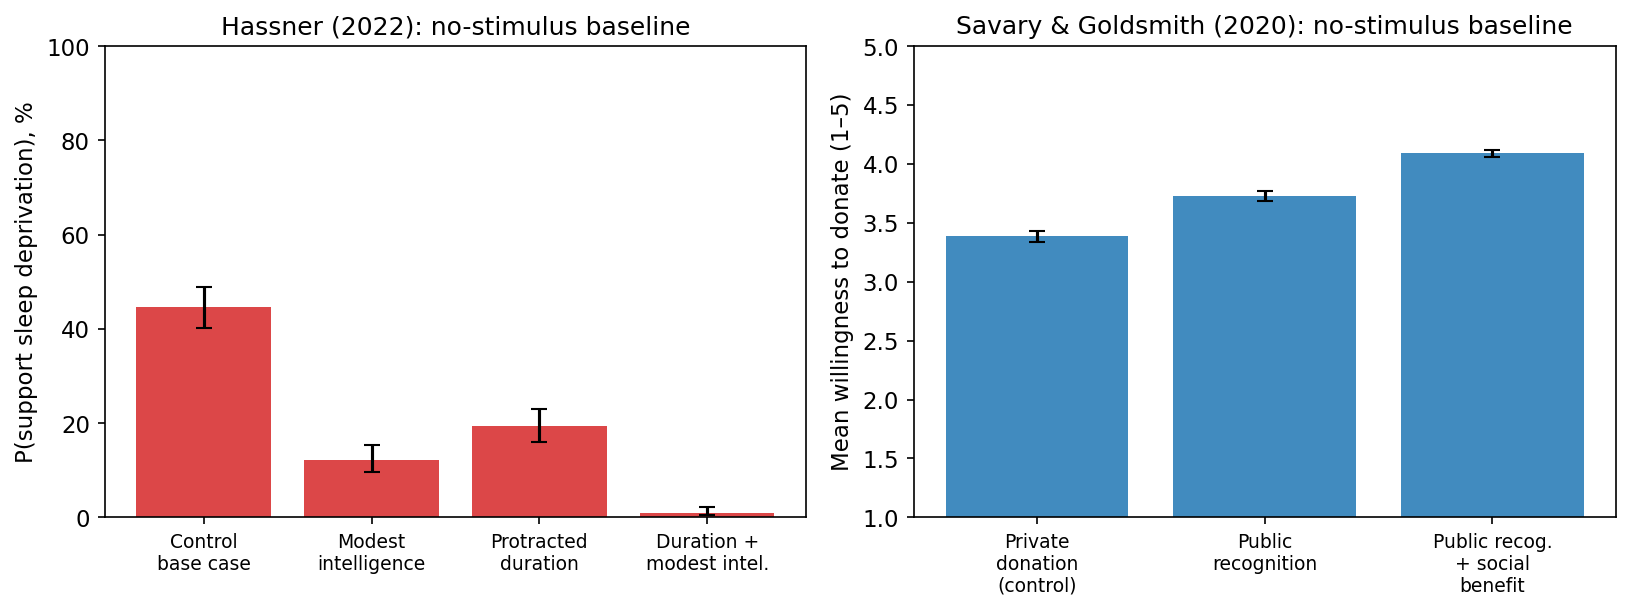
\includegraphics[width=\textwidth]{fig_treatment_replication.png}
\caption{Directional replication of the original treatment effects in the no-stimulus baseline (all four models pooled, $T=0.01$). Left: share of support for sleep deprivation by condition, Wilson 95\% CIs. Right: mean stated willingness to donate by condition, bootstrap 95\% CIs.}
\label{fig:replication}
\end{figure}

\textbf{Stimuli are the strongest factor in the dataset (H2 supported, direction domain-specific).} Omnibus tests of the stimulus factor are significant in all seven treatment groups; pairwise stimulus-vs-baseline contrasts are significant in 31/32 (Hassner) and 24/24 (Savary) comparisons (Figure~\ref{fig:stimuli-effects}). Crucially, the direction is structurally different between the two domains: in Hassner every stimulus \emph{raises} the socially undesirable answer (P(Yes) on the GLM+Kimi subsample: 0.37 baseline $\to$ 0.56--0.64 under the negative-framing family, 0.86 under A, 0.88--0.90 under the positive-framing family), whereas in Savary every stimulus \emph{lowers} stated willingness (3.72 baseline $\to$ 3.14--3.35), i.e., deflates the virtue-signaling pole. In both cases the movement is away from the socially desirable answer --- the stimuli do what they were designed to do, in opposite normative directions.

\begin{figure}[H]
\centering
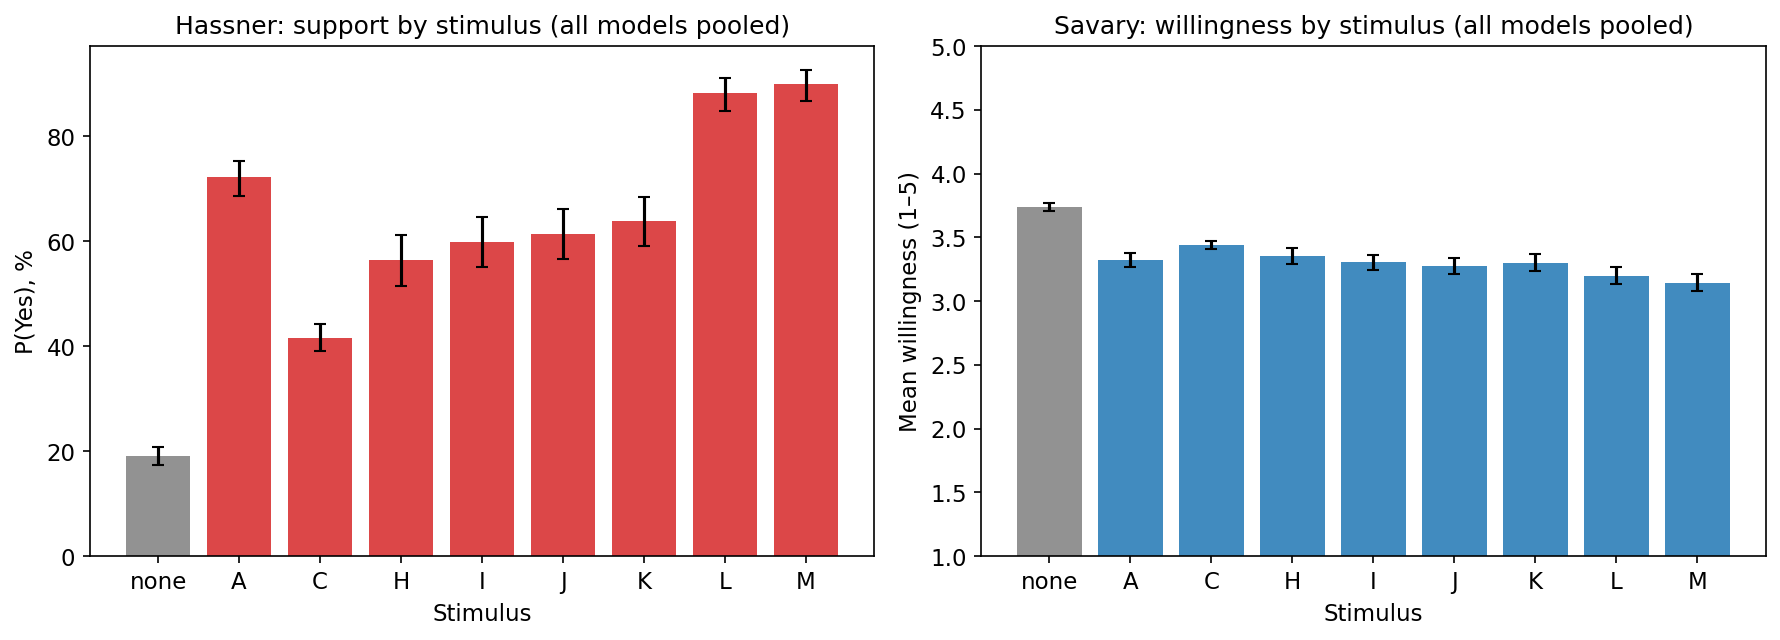
\includegraphics[width=\textwidth]{fig_stimulus_effects.png}
\caption{Final answers by system-prompt stimulus, pooled over treatment groups and models (grey = no-stimulus baseline; 95\% CIs). Every stimulus moves the answer away from the socially desirable pole: upward in Hassner (left), downward in Savary (right). Stimuli H--M are available only for GLM-4.6 and Kimi, which contributes to level differences across bars.}
\label{fig:stimuli-effects}
\end{figure}

\textbf{Stimuli moderate treatment effects (H3 partially supported).} Difference-in-differences contrasts are significant after Holm correction in 11/24 (Hassner) and 10/16 (Savary) pairs, and the moderation is bidirectional: the harsh core stimulus A compresses Hassner treatment effects (its average marginal effect, +49 p.p.\ on P(Yes), is comparable in magnitude to the largest treatment effect of $-54$ p.p.), while the negative-framing family H--K leaves treatment sensitivity largely intact.

\textbf{Stimulus anatomy: valence is the active ingredient (H4 supported).} Regressing answers on stimulus attributes (GLM+Kimi subsample, cluster-robust SE; Table~\ref{tab:attr}) shows that framing valence is the only consistently significant design dimension, and its effect is symmetric across the two domains: positive framing moves answers further from the sanitized baseline than negative framing in Hassner ($\beta = +2.71$ on the logit scale, OR $\approx 15$, $p < 0.0001$) \emph{and} in Savary ($\beta = -0.13$, $p = 0.02$). The identity of the recipient of consequences and of the beneficiary is immaterial. Instruction force matters in the negative domain: the harsh variant A is markedly stronger than the balanced variant C in Hassner ($\beta = 3.99$ vs.\ $1.40$ against baseline) but only slightly stronger in Savary ($-0.48$ vs.\ $-0.36$). A within-factorial refit (H--M only) reproduces all estimates. The earlier working observations --- ``positive framing works better,'' ``the recipient does not matter'' --- are thereby converted from impressions into estimates.

\begin{table}[H]
\centering
\caption{Stimulus-attribute decomposition (GLM+Kimi subsample; cluster-robust SE, cluster = model $\times$ group $\times$ stimulus; reference: no stimulus / negative framing / science / personal beneficiary)}
\label{tab:attr}
\begin{tabular}{L{5.6cm} rrr rrr}
\toprule
 & \multicolumn{3}{c}{\textbf{Hassner (logit)}} & \multicolumn{3}{c}{\textbf{Savary (OLS)}} \\
\cmidrule(lr){2-4}\cmidrule(lr){5-7}
\textbf{Attribute} & $\beta$ & OR & $p$ & $\beta$ & & $p$ \\
\midrule
Positive valence (L/M vs.\ H--K) & $+2.71$ & 15.0 & $<0.001$ & $-0.13$ & & 0.020 \\
Recipient: company vs.\ science & $+0.35$ & 1.42 & 0.060 & $-0.05$ & & 0.34 \\
Beneficiary: public vs.\ personal & $+0.20$ & 1.22 & 0.30 & $-0.01$ & & 0.86 \\
A (harsh core) vs.\ baseline & $+3.99$ & 53.9 & $<0.001$ & $-0.48$ & & $<0.001$ \\
C (balanced) vs.\ baseline & $+1.40$ & 4.05 & $<0.001$ & $-0.36$ & & $<0.001$ \\
H--M family level (H) vs.\ baseline & $+1.44$ & 4.21 & $<0.001$ & $-0.38$ & & $<0.001$ \\
\midrule
$n$ (clusters) & \multicolumn{3}{c}{4{,}630 (72)} & \multicolumn{3}{c}{3{,}473 (54)} \\
\bottomrule
\end{tabular}
\end{table}

\textbf{Robust inference.} Under cluster-robust standard errors, all three Hassner treatment contrasts and the stimuli A/C/H survive (6/6 of the previously significant main effects); in Savary 9 of 10 survive, with the balanced stimulus C becoming borderline ($p = 0.062$). The extreme Hassner stimuli (I--M) produce quasi-separated cells (28/96 cells have P(Yes) $\in \{0,1\}$), so their coefficients are reported descriptively rather than as estimated effects. The proportional-odds assumption fails for Savary, so binary and OLS codings carry the inferential weight. All 15 main effects survive FDR correction. Replicate stability is high overall (modal agreement 0.85 Hassner / 0.81 Savary) and is \emph{reduced} by the stimuli --- models become visibly less certain under realism pressure --- while model heterogeneity is large: GLM and Kimi respond to conditions, Minimax and Qwen3.5 exhibit default-answer strategies (near-constant ``No'' and ``3'' respectively) that produce deceptively high agreement with low Fleiss' $\kappa$.

\subsection{Reasoning level: how stimuli reorganize argumentation}

\textbf{The annotated subsample reproduces the behavioral effects}, with reasoning-level condition models reaching pseudo-$R^2 = 0.486$ (Hassner) and $R^2 = 0.419$ (Savary) from experimental conditions alone.

\textbf{Category prevalence.} The most frequent reasoning categories are prioritization of common interests (86\%), means--ends reasoning (81\%), and emotional reasoning (73\%), alongside a dominant rational reasoning style (86\%); explicit self-deception is nearly absent (0.8\%) (Figure~\ref{fig:prevalence}). Social desirability, in other words, is \emph{latent}: the model almost never verbalizes self-presentation motives, but the structure of its argumentation shifts with conditions.

\begin{figure}[H]
\centering
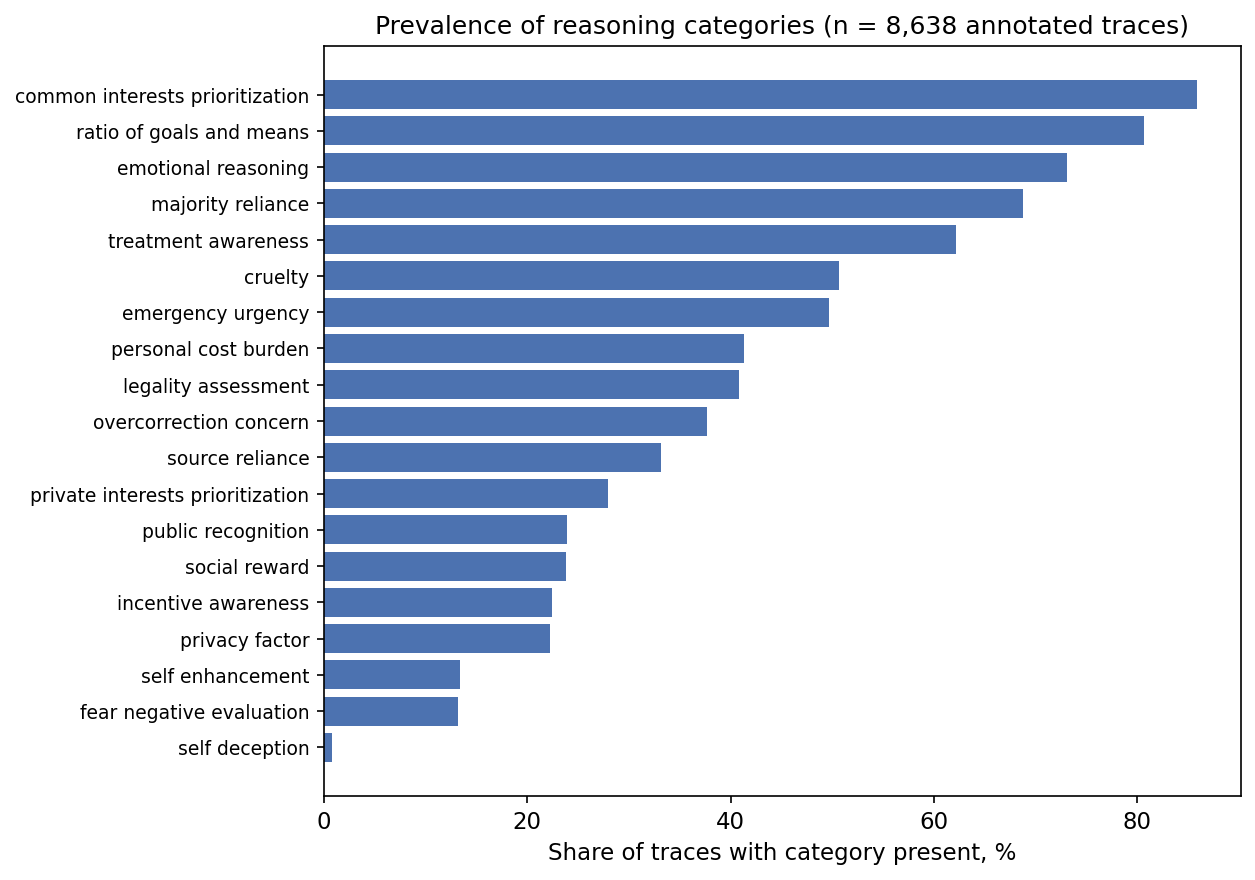
\includegraphics[width=0.86\textwidth]{fig_markup_prevalence.png}
\caption{Prevalence of annotated reasoning categories across the working sample ($n = 8{,}638$ traces; causality variables, binarized).}
\label{fig:prevalence}
\end{figure}

\textbf{The stimulus activates meta-awareness.} The single largest annotation effect is on \texttt{overcorrection\_concern} --- explicit worry about over-shooting toward provocative answers --- which rises from 9\% of baseline traces to 72--76\% under the A/C stimuli (Figure~\ref{fig:overcorrection}). This category is gold-validated ($\kappa = 0.64$), so the finding is measurement-grade. FDR-corrected per-category regressions find broad restructuring: 38/65 condition--category coefficients significant in Hassner and 39/64 in Savary, with the largest stimulus effects on common-interests prioritization and urgency framing in Hassner. The mechanism is two-channel: stimuli simultaneously activate situational arguments (urgency, emotional reasoning) and meta-awareness (overcorrection concern), and the balance of the channels differs between the two experiments --- consistent with the opposite behavioral directions.

\begin{figure}[H]
\centering
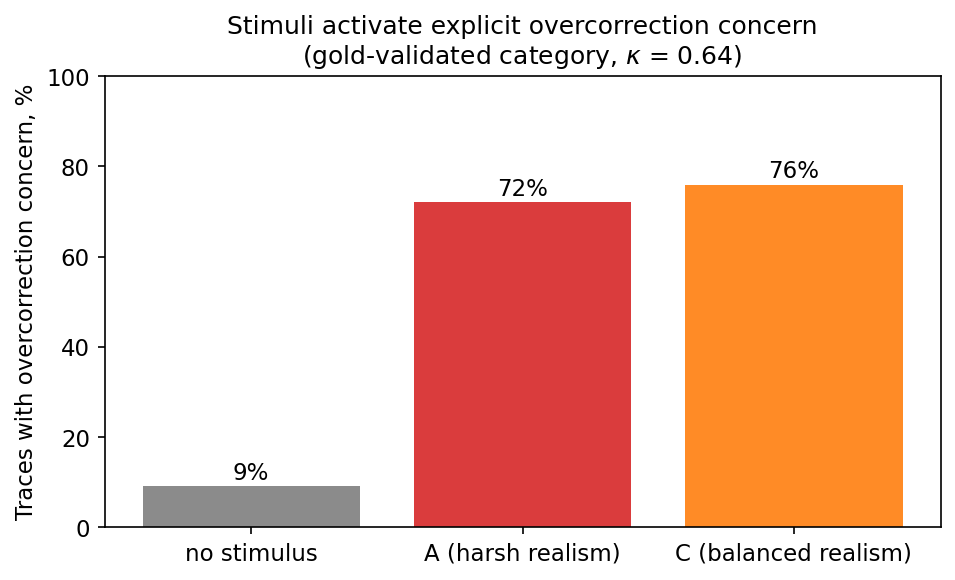
\includegraphics[width=0.7\textwidth]{fig_overcorrection.png}
\caption{Share of reasoning traces containing explicit overcorrection concern, by stimulus condition ($T = 0.01$; all models pooled).}
\label{fig:overcorrection}
\end{figure}

\textbf{Stimulus footprint vs.\ decoding footprint (H5, text level).} Classifiers predicting stimulus presence from annotation features reach cross-validated AUC $= 0.96$ (logit) / $0.97$ (GBM), and still $0.92$ after removing the features that detect the stimulus by construction. By contrast, classifiers predicting the temperature change on no-stimulus runs reach only AUC $= 0.68$--$0.71$ (Figure~\ref{fig:benchmark}). The stimulus thus restructures reasoning far more than a comparable non-semantic perturbation of the generation settings --- the pattern expected if the stimulus enters the reasoning process meaningfully. The harsh and balanced stimulus variants are only moderately separable from each other (AUC $= 0.73$), differing in strength rather than in kind.

\begin{figure}[H]
\centering
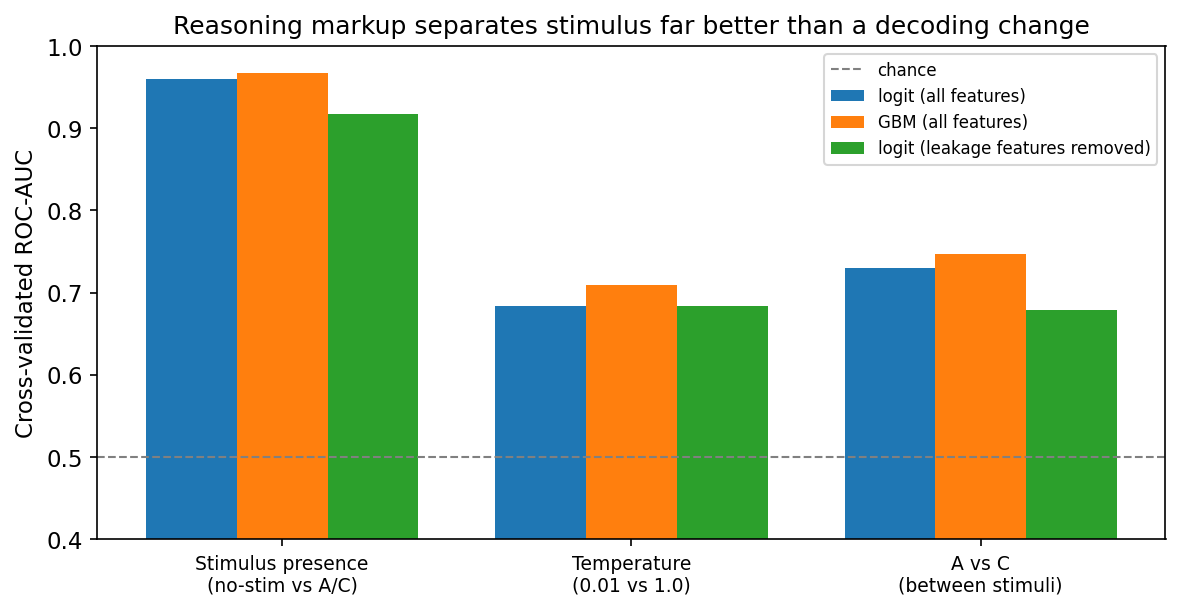
\includegraphics[width=0.82\textwidth]{fig_benchmark.png}
\caption{Separability benchmark on annotation features (stratified 5-fold CV ROC-AUC). The stimulus leaves a far larger footprint in reasoning structure than a change of decoding temperature, and the result survives removal of leakage features (stimulus awareness, stimulus-effect direction).}
\label{fig:benchmark}
\end{figure}

\subsection{Reasoning $\to$ answer: additive in one domain, interactive in the other}

Linking annotation features to final answers raises the Hassner condition model from pseudo-$R^2$ 0.486 to 0.825 and the Savary model from 0.419 to 0.482. The headline Hassner number must be read with care: most of the increment comes from the co-generated stated-position feature, so it quantifies \emph{coherence} between reasoning and answer rather than a causal recipe; the non-tautological increment is on the order of +0.05.

The interpretable-ML diagnostic then yields a clean structural contrast. In Hassner, gradient boosting does not outperform the logit (AUC 0.991 vs.\ 0.989; without condition controls 0.979 vs.\ 0.979): the reasoning$\to$answer mapping is \emph{additive}, and the regression coefficients are its complete interpretable description --- no post hoc attribution is needed. In Savary, the nonlinear model clearly wins (CV $R^2$ 0.558 vs.\ 0.475), so TreeSHAP is applied there in a discovery role (Figure~\ref{fig:shap}). The interaction analysis locates the nonlinearity almost entirely in \emph{interactions with context} rather than between reasoning features, and every discovered pair is re-estimated as an explicit term in a confirmatory OLS with robust inference (Table~\ref{tab:interactions}): the strongest pair, treatment(social benefit) $\times$ no-stimulus, is the reasoning-level echo of the behavioral moderation of H3; privacy-reasoning $\times$ no-stimulus shows that the stimulus changes how privacy arguments convert into answers; the one substantive feature--feature interaction is emotional reasoning $\times$ privacy. Adding the six discovered terms raises the confirmatory OLS $R^2$ from 0.487 to 0.519, with five of six significant. SHAP is thus used in the role this data structure justifies --- discovery on the experiment where nonlinearity demonstrably exists --- with all conclusions anchored in the confirmatory regression; LIME was considered and rejected as unstable on tabular binary features and dominated by SHAP.

\begin{figure}[H]
\centering
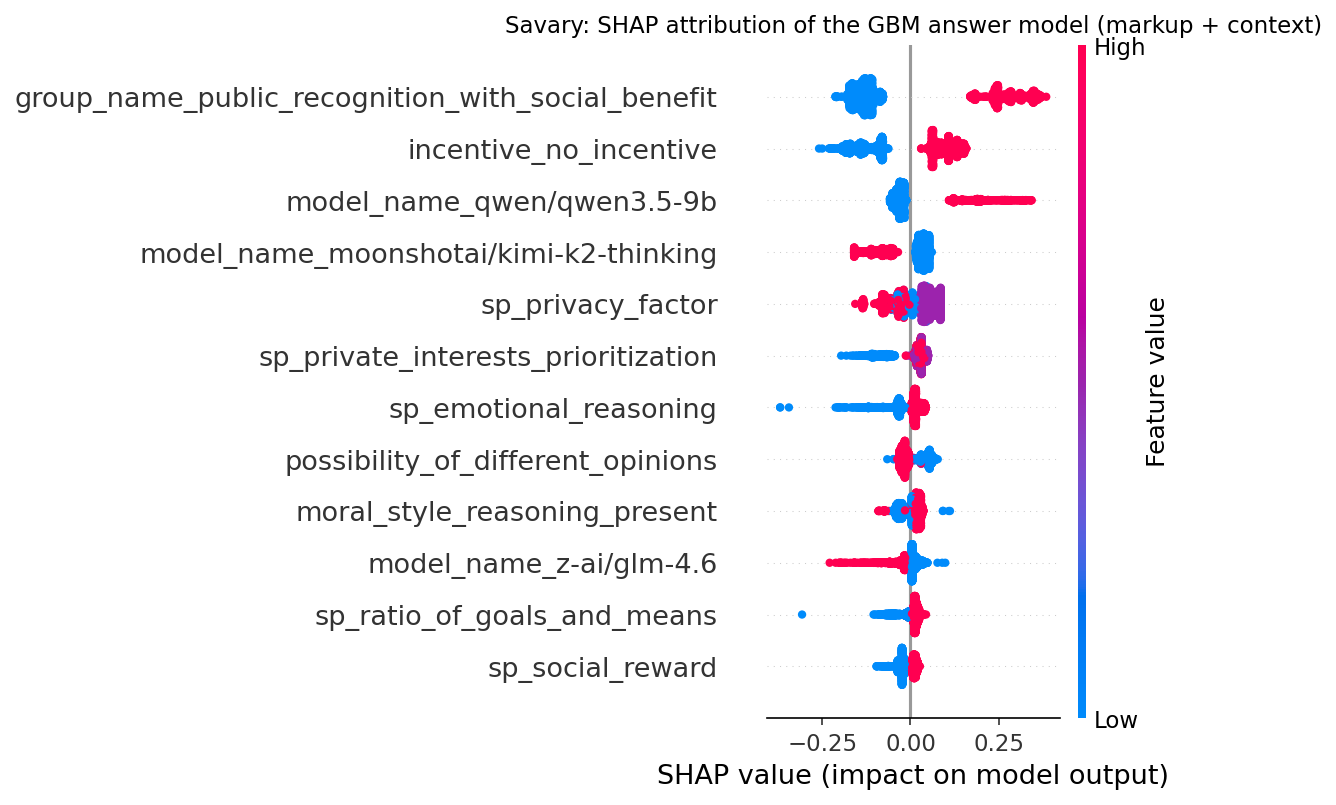
\includegraphics[width=0.92\textwidth]{fig_shap_savary.png}
\caption{SHAP attribution for the Savary gradient-boosting answer model (annotation features + condition controls). Each point is one trace; color encodes the feature value, horizontal position its contribution to the predicted willingness.}
\label{fig:shap}
\end{figure}

\begin{table}[H]
\centering
\caption{SHAP-discovered interactions re-estimated in the confirmatory OLS (Savary; HC3 SE). Base model $R^2 = 0.487$; with interaction terms $R^2 = 0.519$.}
\label{tab:interactions}
\begin{tabular}{L{8.4cm} rr}
\toprule
\textbf{Interaction term} & $\beta$ & $p$ \\
\midrule
treatment(social benefit) $\times$ no-stimulus & $-0.25$ & $<0.001$ \\
privacy reasoning $\times$ no-stimulus & $-0.12$ & $<0.001$ \\
treatment(social benefit) $\times$ Qwen3.5 & $-0.33$ & $<0.001$ \\
no-stimulus $\times$ Kimi & $-0.18$ & $<0.001$ \\
privacy reasoning $\times$ treatment(social benefit) & $+0.01$ & 0.81 \\
emotional reasoning $\times$ privacy reasoning & $+0.08$ & $<0.001$ \\
\bottomrule
\end{tabular}
\end{table}

\subsection{Representational level: hidden states}

\textbf{The stimulus is encoded in mid-layers.} Layer-wise separation between stimulus and no-stimulus runs peaks at layer 20 of 37 (Figure~\ref{fig:separation}; a plateau L20--L21; the argmax lands on L20 in 49.7\% of bootstrap resamples, and separation is significant at every layer). The experiment identity dominates the stimulus as a separating factor, and linear probes confirm a hierarchy: stimulus presence is decodable with perfect balanced accuracy at \emph{all} layers --- including the first, which marks this as a surface text artifact rather than ``semantic'' processing --- whereas abstract \emph{treatment} status is not decodable at all under honest group-held-out validation (LOGO AUC 0.034 at L20, permutation $p = 1.0$): the model represents concrete scenarios, not the experimenter's abstraction of ``being treated.'' Given $n = 98$, only effects of AUC $\gtrsim 0.63$ were detectable, so this null is a bounded one.

\begin{figure}[H]
\centering
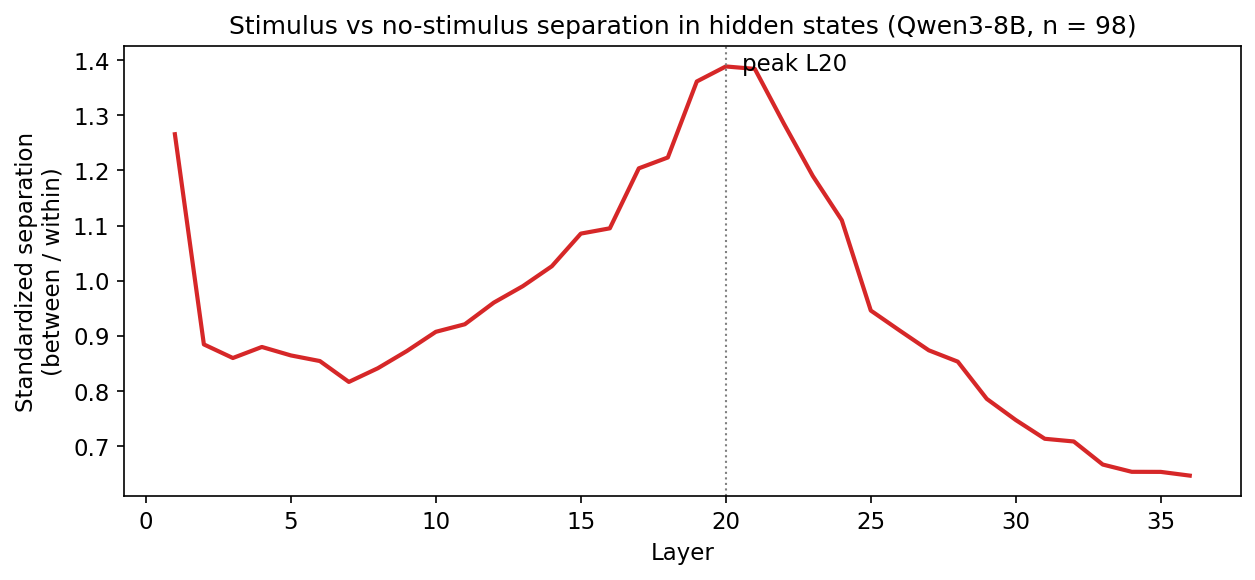
\includegraphics[width=0.85\textwidth]{fig_hs_separation.png}
\caption{Standardized separation (between-condition distance over within-condition dispersion) between stimulus and no-stimulus hidden states, by layer. Local Qwen3-8B, last-token representations, $n = 98$ runs.}
\label{fig:separation}
\end{figure}

\textbf{Stimuli shorten the computational trajectory.} The cumulative layer-to-layer trajectory length of the representation is significantly shorter under stimuli (3{,}370 vs.\ 3{,}444 units; paired Wilcoxon on matched scenarios, $p = 1.2\times10^{-4}$), with the deficit accumulating from mid-layers onward (Figure~\ref{fig:trajectory}): the stimulus frame pre-structures the computation, leaving the late layers less work --- consistent with the meta-awareness channel found in the reasoning track.

\begin{figure}[H]
\centering
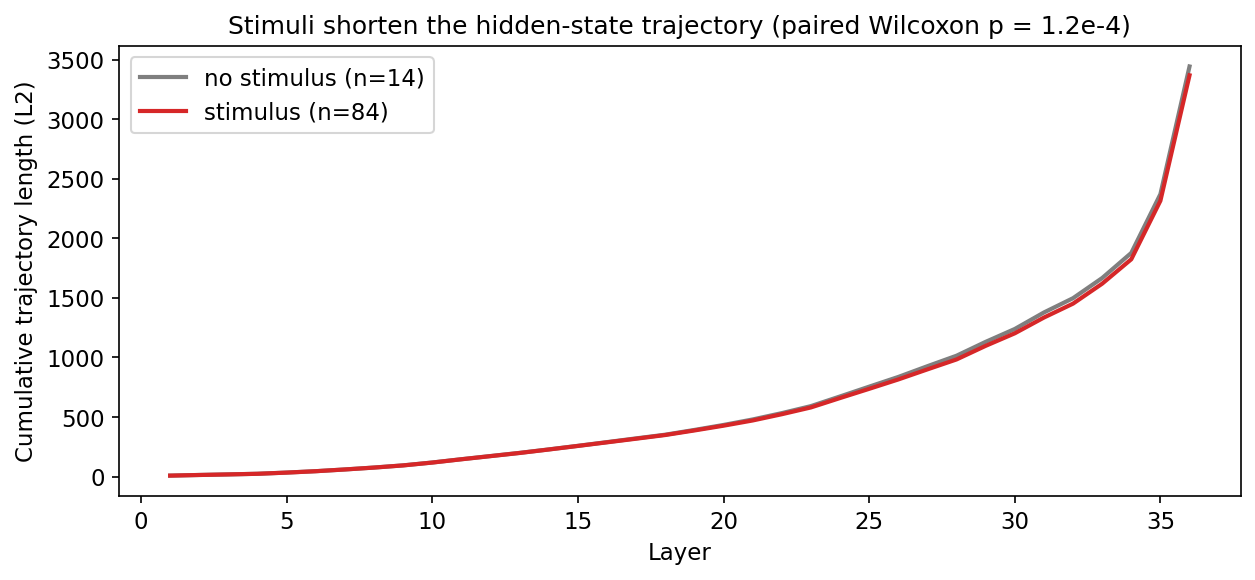
\includegraphics[width=0.85\textwidth]{fig_hs_trajectory.png}
\caption{Cumulative hidden-state trajectory length across layers, by condition. Stimulus runs traverse a shorter path, with the gap accumulating from the mid-layers onward.}
\label{fig:trajectory}
\end{figure}

\textbf{Representation and behavior dissociate (H5 supported in its strong form).} The local model is behaviorally degenerate in both experiments --- in Hassner it answers Yes with P $\approx 0.998$ regardless of condition; in Savary the stimulus \emph{lowers} expected willingness (3.89 $\to$ 3.07--3.29), the reverse of the API models' positive pole --- yet its hidden-state shift at L20 is of the same magnitude ($\approx$16 units) in both experiments, despite a $\sim$700$\times$ difference in the behavioral effect. The model can register a stimulus representationally while not acting on it behaviorally: representational sensitivity does not license behavioral predictions.

\textbf{Answer decodability rises late (exploratory).} On Savary (the non-degenerate case; $n = 42$), ridge probes decode the continuous answer from every layer (LOO $R^2 = 0.86$ at L2, rising monotonically to 0.99 at L28--30; permutation $p \approx 0.005$), but the pooled curve is dominated by condition identity, which is itself prompt-visible. The informative quantity is the condition-residualized probe (Figure~\ref{fig:decodability}): the within-condition component of the answer (7\% of variance) is decodable at $R^2 \approx 0.55$ from early layers and peaks at $R^2 \approx 0.66$ at layers 27--30 --- \emph{later} than the stimulus-separation peak at L20. The picture is consistent across analyses: the stimulus is processed in mid-layers, the answer crystallizes in late layers.

\begin{figure}[H]
\centering
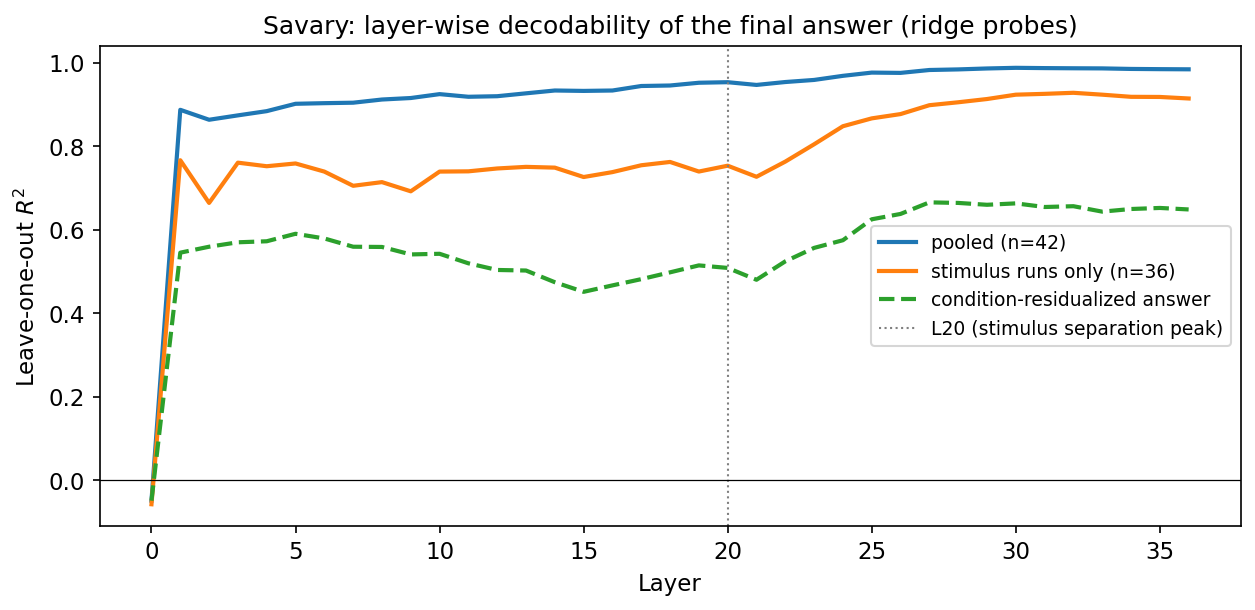
\includegraphics[width=0.85\textwidth]{fig_hs_decodability.png}
\caption{Layer-wise decodability of the final answer in Savary (ridge probes, leave-one-out $R^2$). The pooled and stimulus-only curves are inflated by prompt-visible condition identity; the condition-residualized curve (dashed) isolates answer information beyond the condition and peaks after the stimulus-separation layer L20.}
\label{fig:decodability}
\end{figure}

\subsection{Summary of results against hypotheses}

\begin{table}[H]
\centering
\caption{Hypotheses and outcomes}
\begin{tabular}{L{1.2cm} L{8.2cm} L{4.6cm}}
\toprule
 & \textbf{Hypothesis} & \textbf{Outcome} \\
\midrule
H1 & Directional replication of treatment effects & Supported (4/4 directions) \\
H2 & Stimuli shift answers from the desirable pole & Supported; direction is domain-specific and symmetric in desirability terms \\
H3 & Stimuli moderate treatment effects & Partially supported ($\approx$50\% of DiD pairs; bidirectional) \\
H4 & Positive framing $>$ negative framing & Supported in both experiments; recipient/beneficiary identity immaterial \\
H5 & Stimulus visible below the answer surface & Supported: reasoning AUC 0.96 vs.\ 0.68 temperature benchmark; mid-layer encoding; representation--behavior dissociation \\
\bottomrule
\end{tabular}
\end{table}

\section{MoralLens: a Fine-Tuned Annotation Model}

% ============================================================
% TODO: this chapter is intentionally left empty.
% To be completed by the authors: description of the fine-tuned
% MoralLens annotation model (training data construction, base model,
% fine-tuning setup, evaluation metrics, agreement with gold labels,
% comparison against the gpt-5.4-mini pilot annotator).
% ============================================================

\emph{[This chapter will describe the fine-tuned MoralLens model for structured annotation of reasoning traces and is to be completed.]}

\section{Scope and Limitations}

Several limits of the present study should be made explicit.

\begin{itemize}
    \item \textbf{Corpus breadth.} The empirical corpus contains two attitude-expression experiments; the methodological and self-report SDB categories remain outside the current scope, and generalization beyond attitude expression is untested.
    \item \textbf{Design imbalance.} The H--M stimulus family was fielded only on GLM-4.6 and Kimi; the stimulus-anatomy estimates are conditional on this two-model subsample. Completing the model $\times$ stimulus grid is the most direct planned extension.
    \item \textbf{Annotation reliability is uneven.} Only \texttt{cruelty} ($\kappa = 1.0$) and \texttt{overcorrection\_concern} ($\kappa = 0.64$) are gold-validated; several psychologically subtle categories code at chance level, and findings resting on them are exploratory. The gold subset ($n=27$) is itself small.
    \item \textbf{Cross-population stitching.} The three tracks observe different model populations (four API models; a fifth local model for hidden states; a sixth model as annotator). The representational findings, including the dissociation result, are established on one local model with $n = 98$ runs and last-token representations only.
    \item \textbf{Behavioral degeneracy of the local model.} Hassner is saturated (P(Yes) $\approx 0.998$) and Savary is direction-reversed for the local model, which limits which representational questions are answerable and marks the stimulus-direction reversal as potentially model-specific.
    \item \textbf{Inference granularity.} The effective number of independent observations is the number of design cells, not rows; all headline claims are therefore tied to the cluster-robust estimates, and quasi-separated cells are reported descriptively.
    \item \textbf{No demographic conditioning.} Respondent profiles are deliberately absent from the prompts; the project measures the ``blank respondent'' regime, and interactions between stimuli and persona conditioning remain future work.
\end{itemize}

\section{Conclusion}

This project asked how large language models react to stimuli in vignette-based survey experiments shaped by social desirability bias, and answered it on three levels of observation within a single controlled design: 15{,}680 behavioral runs of four reasoning-capable API models on two opposite-valence published experiments, 10{,}080 LLM-annotated reasoning traces, and 98 white-box runs of a local model with full hidden-state extraction.

Three results carry the main weight. First, LLMs reproduce the direction of all four original treatment effects in the baseline, while realism-oriented system-prompt stimuli move answers away from the socially desirable pole in both domains --- raising support for coercive interrogation and deflating overstated willingness to donate --- and the decomposition of the stimulus inventory shows that \emph{framing valence}, not the identity of who benefits or suffers, is the active design ingredient: positively framed realism instructions outperform penalty framing symmetrically across domains. Second, the stimulus restructures the reasoning process itself: it activates explicit overcorrection concern (9\% $\to$ 72--76\% of traces; gold-validated), shifts the argumentative repertoire, and leaves a footprint in annotated reasoning that classifiers separate at AUC 0.96 --- far above the 0.68 footprint of a comparable decoding-settings change. Third, the levels do not reduce to one another: the local model encodes the stimulus in mid-layer representations (peak at layer 20) and shortens its computational trajectory under stimuli, while its behavior barely moves --- representational sensitivity and behavioral sensitivity dissociate, and the answer itself becomes decodable latest in the network, after the stimulus has been processed.

For the practical question that motivated the project --- can LLMs serve as pilot environments for survey experiments in SDB-sensitive domains --- the answer is a qualified yes. The models are usable for \emph{directional, within-design piloting}: treatment contrasts replicate, stimulus interventions behave lawfully enough to be designed (valence matters, recipients do not), and the reasoning traces provide a measurable window into the response process. The qualifications are equally clear: absolute response levels are not trustworthy, model heterogeneity is large enough that any single-model pilot is uninformative, and what a model represents internally is not what it will do. A survey methodologist using LLM piloting should therefore read it the way this project does --- as a source of contrasts, mechanisms, and fragility warnings, not of numbers.

\newpage
\begin{thebibliography}{99}

\bibitem[Aher et al.(2023)]{aher2023}
Aher, G. V., Arriaga, R. I., \& Kalai, A. T. (2023). Using large language models to simulate multiple humans and replicate human subject studies. \textit{Proceedings of the 40th International Conference on Machine Learning (ICML)}, PMLR 202, 337--371.

\bibitem[Alain \& Bengio(2016)]{alain2016}
Alain, G., \& Bengio, Y. (2016). Understanding intermediate layers using linear classifier probes. \textit{arXiv preprint} arXiv:1610.01644.

\bibitem[Argyle et al.(2023)]{argyle2023}
Argyle, L. P., Busby, E. C., Fulda, N., Gubler, J. R., Rytting, C., \& Wingate, D. (2023). Out of one, many: Using language models to simulate human samples. \textit{Political Analysis}, 31(3), 337--351.

\bibitem[Belinkov(2022)]{belinkov2022}
Belinkov, Y. (2022). Probing classifiers: Promises, shortcomings, and advances. \textit{Computational Linguistics}, 48(1), 207--219.

\bibitem[Bisbee et al.(2024)]{bisbee2024}
Bisbee, J., Clinton, J. D., Dorff, C., Kenkel, B., \& Larson, J. M. (2024). Synthetic replacements for human survey data? The perils of large language models. \textit{Political Analysis}, 32(4), 401--416.

\bibitem[Blair \& Imai(2012)]{blair2012}
Blair, G., \& Imai, K. (2012). Statistical analysis of list experiments. \textit{Political Analysis}, 20(1), 47--77.

\bibitem[Burns et al.(2023)]{burns2022}
Burns, C., Ye, H., Klein, D., \& Steinhardt, J. (2023). Discovering latent knowledge in language models without supervision. \textit{Proceedings of the 11th International Conference on Learning Representations (ICLR)}.

\bibitem[Crowne \& Marlowe(1960)]{crowne1960}
Crowne, D. P., \& Marlowe, D. (1960). A new scale of social desirability independent of psychopathology. \textit{Journal of Consulting Psychology}, 24(4), 349--354.

\bibitem[Dillion et al.(2023)]{dillion2023}
Dillion, D., Tandon, N., Gu, Y., \& Gray, K. (2023). Can AI language models replace human participants? \textit{Trends in Cognitive Sciences}, 27(7), 597--600.

\bibitem[Dominguez-Olmedo et al.(2024)]{dominguez2024}
Dominguez-Olmedo, R., Hardt, M., \& Mendler-D\"unner, C. (2024). Questioning the survey responses of large language models. \textit{Advances in Neural Information Processing Systems 37 (NeurIPS)}.

\bibitem[Gilardi et al.(2023)]{gilardi2023}
Gilardi, F., Alizadeh, M., \& Kubli, M. (2023). ChatGPT outperforms crowd workers for text-annotation tasks. \textit{Proceedings of the National Academy of Sciences}, 120(30), e2305016120.

\bibitem[Grossmann et al.(2023)]{grossmann2023}
Grossmann, I., Feinberg, M., Parker, D. C., Christakis, N. A., Tetlock, P. E., \& Cunningham, W. A. (2023). AI and the transformation of social science research. \textit{Science}, 380(6650), 1108--1109.

\bibitem[Hassner(2022)]{hassner2022}
Hassner, R. E. (2022). Persuasive and unpersuasive critiques of torture. \textit{Perspectives on Politics}, 20(4), 1255--1268.

\bibitem[Hewitt \& Liang(2019)]{hewitt2019}
Hewitt, J., \& Liang, P. (2019). Designing and interpreting probes with control tasks. \textit{Proceedings of EMNLP-IJCNLP 2019}, 2733--2743.

\bibitem[Horton et al.(2023)]{horton2023}
Horton, J. J., Filippas, A., \& Manning, B. S. (2023). Large language models as simulated economic agents: What can we learn from homo silicus? \textit{NBER Working Paper No.\ 31122}.

\bibitem[Krumpal(2013)]{krumpal2013}
Krumpal, I. (2013). Determinants of social desirability bias in sensitive surveys: A literature review. \textit{Quality \& Quantity}, 47(4), 2025--2047.

\bibitem[Lundberg \& Lee(2017)]{lundberg2017}
Lundberg, S. M., \& Lee, S.-I. (2017). A unified approach to interpreting model predictions. \textit{Advances in Neural Information Processing Systems 30 (NeurIPS)}.

\bibitem[Nederhof(1985)]{nederhof1985}
Nederhof, A. J. (1985). Methods of coping with social desirability bias: A review. \textit{European Journal of Social Psychology}, 15(3), 263--280.

\bibitem[Park et al.(2023)]{park2023}
Park, J. S., O'Brien, J. C., Cai, C. J., Morris, M. R., Liang, P., \& Bernstein, M. S. (2023). Generative agents: Interactive simulacra of human behavior. \textit{Proceedings of the 36th Annual ACM Symposium on User Interface Software and Technology (UIST)}.

\bibitem[Paulhus(1984)]{paulhus1984}
Paulhus, D. L. (1984). Two-component models of socially desirable responding. \textit{Journal of Personality and Social Psychology}, 46(3), 598--609.

\bibitem[R\"ottger et al.(2024)]{rottger2024}
R\"ottger, P., Kirk, H. R., Vidgen, B., Attanasio, G., Bianchi, F., \& Hovy, D. (2024). Political compass or spinning arrow? Towards more meaningful evaluations for values and opinions in large language models. \textit{Proceedings of the 62nd Annual Meeting of the Association for Computational Linguistics (ACL)}.

\bibitem[Salecha et al.(2024)]{salecha2024}
Salecha, A., Ireland, M. E., Subrahmanya, S., Sedoc, J., Ungar, L. H., \& Eichstaedt, J. C. (2024). Large language models display human-like social desirability biases in Big Five personality surveys. \textit{PNAS Nexus}, 3(12), pgae533.

\bibitem[Santurkar et al.(2023)]{santurkar2023}
Santurkar, S., Durmus, E., Ladhak, F., Lee, C., Liang, P., \& Hashimoto, T. (2023). Whose opinions do language models reflect? \textit{Proceedings of the 40th International Conference on Machine Learning (ICML)}, PMLR 202, 29971--30004.

\bibitem[Savary \& Goldsmith(2020)]{savary2020}
Savary, J., \& Goldsmith, K. (2020). Unobserved altruism: How self-signaling motivations and social benefits shape willingness to donate. \textit{Journal of Experimental Psychology: Applied}, 26(3), 538--550.

\bibitem[Sharma et al.(2024)]{sharma2023}
Sharma, M., Tong, M., Korbak, T., Duvenaud, D., Askell, A., Bowman, S. R., et al. (2024). Towards understanding sycophancy in language models. \textit{Proceedings of the 12th International Conference on Learning Representations (ICLR)}.

\bibitem[T\"ornberg(2024)]{tornberg2024}
T\"ornberg, P. (2024). Best practices for text annotation with large language models. \textit{Sociologica}, 18(1).

\bibitem[Tourangeau \& Yan(2007)]{tourangeau2007}
Tourangeau, R., \& Yan, T. (2007). Sensitive questions in surveys. \textit{Psychological Bulletin}, 133(5), 859--883.

\bibitem[Zou et al.(2023)]{zou2023}
Zou, A., Phan, L., Chen, S., Campbell, J., Guo, P., Ren, R., et al. (2023). Representation engineering: A top-down approach to AI transparency. \textit{arXiv preprint} arXiv:2310.01405.

\end{thebibliography}

\end{document}
